% Options for packages loaded elsewhere
\PassOptionsToPackage{unicode}{hyperref}
\PassOptionsToPackage{hyphens}{url}
%
\documentclass[
  ignorenonframetext,
]{beamer}
\usepackage{pgfpages}
\setbeamertemplate{caption}[numbered]
\setbeamertemplate{caption label separator}{: }
\setbeamercolor{caption name}{fg=normal text.fg}
\beamertemplatenavigationsymbolsempty
% Prevent slide breaks in the middle of a paragraph
\widowpenalties 1 10000
\raggedbottom
\setbeamertemplate{part page}{
  \centering
  \begin{beamercolorbox}[sep=16pt,center]{part title}
    \usebeamerfont{part title}\insertpart\par
  \end{beamercolorbox}
}
\setbeamertemplate{section page}{
  \centering
  \begin{beamercolorbox}[sep=12pt,center]{part title}
    \usebeamerfont{section title}\insertsection\par
  \end{beamercolorbox}
}
\setbeamertemplate{subsection page}{
  \centering
  \begin{beamercolorbox}[sep=8pt,center]{part title}
    \usebeamerfont{subsection title}\insertsubsection\par
  \end{beamercolorbox}
}
\AtBeginPart{
  \frame{\partpage}
}
\AtBeginSection{
  \ifbibliography
  \else
    \frame{\sectionpage}
  \fi
}
\AtBeginSubsection{
  \frame{\subsectionpage}
}
\usepackage{amsmath,amssymb}
\usepackage{lmodern}
\usepackage{iftex}
\ifPDFTeX
  \usepackage[T1]{fontenc}
  \usepackage[utf8]{inputenc}
  \usepackage{textcomp} % provide euro and other symbols
\else % if luatex or xetex
  \usepackage{unicode-math}
  \defaultfontfeatures{Scale=MatchLowercase}
  \defaultfontfeatures[\rmfamily]{Ligatures=TeX,Scale=1}
\fi
% Use upquote if available, for straight quotes in verbatim environments
\IfFileExists{upquote.sty}{\usepackage{upquote}}{}
\IfFileExists{microtype.sty}{% use microtype if available
  \usepackage[]{microtype}
  \UseMicrotypeSet[protrusion]{basicmath} % disable protrusion for tt fonts
}{}
\makeatletter
\@ifundefined{KOMAClassName}{% if non-KOMA class
  \IfFileExists{parskip.sty}{%
    \usepackage{parskip}
  }{% else
    \setlength{\parindent}{0pt}
    \setlength{\parskip}{6pt plus 2pt minus 1pt}}
}{% if KOMA class
  \KOMAoptions{parskip=half}}
\makeatother
\usepackage{xcolor}
\newif\ifbibliography
\setlength{\emergencystretch}{3em} % prevent overfull lines
\providecommand{\tightlist}{%
  \setlength{\itemsep}{0pt}\setlength{\parskip}{0pt}}
\setcounter{secnumdepth}{-\maxdimen} % remove section numbering
\newlength{\cslhangindent}
\setlength{\cslhangindent}{1.5em}
\newlength{\csllabelwidth}
\setlength{\csllabelwidth}{3em}
\newlength{\cslentryspacingunit} % times entry-spacing
\setlength{\cslentryspacingunit}{\parskip}
\newenvironment{CSLReferences}[2] % #1 hanging-ident, #2 entry spacing
 {% don't indent paragraphs
  \setlength{\parindent}{0pt}
  % turn on hanging indent if param 1 is 1
  \ifodd #1
  \let\oldpar\par
  \def\par{\hangindent=\cslhangindent\oldpar}
  \fi
  % set entry spacing
  \setlength{\parskip}{#2\cslentryspacingunit}
 }%
 {}
\usepackage{calc}
\newcommand{\CSLBlock}[1]{#1\hfill\break}
\newcommand{\CSLLeftMargin}[1]{\parbox[t]{\csllabelwidth}{#1}}
\newcommand{\CSLRightInline}[1]{\parbox[t]{\linewidth - \csllabelwidth}{#1}\break}
\newcommand{\CSLIndent}[1]{\hspace{\cslhangindent}#1}
\ifLuaTeX
  \usepackage{selnolig}  % disable illegal ligatures
\fi
\IfFileExists{bookmark.sty}{\usepackage{bookmark}}{\usepackage{hyperref}}
\IfFileExists{xurl.sty}{\usepackage{xurl}}{} % add URL line breaks if available
\urlstyle{same} % disable monospaced font for URLs
\hypersetup{
  pdftitle={Introduction to Duration Models},
  pdfauthor={Sreeram Anantharaman},
  hidelinks,
  pdfcreator={LaTeX via pandoc}}

\title{Introduction to Duration Models}
\author{Sreeram Anantharaman}
\date{2022-11-14}

\begin{document}
\frame{\titlepage}

\begin{frame}{Introduction}
\protect\hypertarget{introduction}{}
\begin{itemize}
\item
  Duration models are concerned with time intervals between events.
\item
  Engle and Russell (\protect\hyperlink{ref-ACD}{1998}) introduced the
  Autoregressive Conditional Duration model, which presents a new way of
  modelling random durations arising from high frequency data.
\item
  ACD models were developed to study the dynamic structure of durations
  in the context of irregularly spaced financial transactions data.
\item
  The model treats the time between events as a stochastic process and
  proposes a new class of point processes with dependent arrival rates.
\end{itemize}
\end{frame}

\begin{frame}{Introduction (Cont..)}
\protect\hypertarget{introduction-cont..}{}
\begin{itemize}
\item
  This presentation provides an overview of different techniques to
  model durations.
\item
  Several simulation studies are presented for different types of
  Log-ACD models.
\item
  We have also shown an example where a log-ACD model is fit to wave
  height durations which is a very different example of the application.
\end{itemize}
\end{frame}

\begin{frame}{Background}
\protect\hypertarget{background}{}
\begin{itemize}
\item
  The Autoregressive Conditional Heteroskedasticity (ARCH) and
  Generalized Autoregressive Conditional Heteroskedasticity (GARCH)
  models are considered an important modeling tool if the goal of the
  study is to analyze and forecast volatility in a data especially in
  financial applications.
\item
  In a linear regression the variances of the error terms are assumed to
  be constant throughout the data.
\item
  If this is not satisfied then we say the data is affected by
  Heteroskedasticity.
\item
  In that case linear model may not provide precise conclusions.
\item
  This situation is tackled by the ARCH/GARCH framework which models
  these variances.
\end{itemize}
\end{frame}

\begin{frame}{Relationship between GARCH and ACD}
\protect\hypertarget{relationship-between-garch-and-acd}{}
\begin{itemize}
\item
  Several models have been developed from the ARCH/GARCH models.
\item
  One such model is the Autoregressive Conditional Duration (ACD) model.
\item
  Especially the ACD model is considered as an counterpart of the GARCH
  model.
\item
  The ACD model is used to analyze the financial durations rather than
  the returns.
\item
  That is, instead of modeling the conditional variances we model the
  conditional mean of the durations.
\end{itemize}
\end{frame}

\begin{frame}{Motivation for Duration Models}
\protect\hypertarget{motivation-for-duration-models}{}
\begin{itemize}
\item
  Longer duration indicate lack of trading activity which implies that
  there is no new information.
\item
  Arrival of new information leads to more activity which in turn
  implies shorter durations.
\item
  Thus the behaviour of the durations provide useful information about
  the market.
\end{itemize}
\end{frame}

\hypertarget{types-of-duration-models}{%
\section{Types of Duration Models}\label{types-of-duration-models}}

\begin{frame}{ACD Model}
\protect\hypertarget{acd-model}{}
\begin{itemize}
\tightlist
\item
  The ACD model are defined in terms of conditional density of
  durations.
\end{itemize}

The \(i^{th}\) duration is defined as time interval between the events
occuring at time \(t_i\) and \(t_{i-1}\):

\(x_i = t_i - t_{i-1}\).

ACD model assumes that the time dependence between the \(i^{th}\)
duration and prior durations is completely explained by \(\psi_i\).

Let \(\psi_i\) be the expectation of the \(i^{th}\) duration then we
have,

\(E(x_i | x_{i-1}, ..., x_1) = \psi_i\).
\end{frame}

\begin{frame}{ACD Model (Cont..)}
\protect\hypertarget{acd-model-cont..}{}
Then the durations \(x_i\) can be written as:

\(x_i = \psi_i \epsilon_i\) ;

where \(\epsilon_i\) are i.i.d non negative random variable with
\(E(\epsilon_i)=1\) and density function \(f_{\epsilon}\) , and,

\(\psi_i = \omega + \sum_{j=1}^m \alpha_j x_{i-j} + \sum_{j=1}^q \beta_j \psi_{i-j}\)
;

with the following constraints on the coefficients:

\(\omega > 0\), \(\beta \geq 0\), \(\alpha \geq 0\)

and \(\sum_{j=1}^m\alpha + \sum_{j=1}^q\beta < 1\) to ensure
non-negativity and weak stationarity of the durations \(x_i\).

This is called an ACD(\(m, q\)) where the \(m\) and \(q\) refer to the
orders of the lags.
\end{frame}

\begin{frame}{SCD Model}
\protect\hypertarget{scd-model}{}
\begin{itemize}
\tightlist
\item
  Stochastic Conditional duration (SCD) Model was proposed by Bauwens
  and Veredas (\protect\hyperlink{ref-SCD}{2004}) and is based on the
  assumption that there exists a stochastic latent variable that
  generates the durations.
\end{itemize}

The generalized form of the SCD model is:

\(x_i = e^{\psi_i} \epsilon_i\) ;

where \(\epsilon_i ~\) i.i.d with \(E(\epsilon_i)=1\), and,

\(\psi_i = \omega + \sum_{j=0}^m \alpha_j x_{i-j} + \sum_{j=0}^q \beta_j \psi_{i-j} + z_i\)
;

where \(z_i\) \textasciitilde{} iid \(N(0,\sigma_z^2)\) and \(z_i\) and
\(\epsilon_i\) are independent.

The conditional expected duration, which was a fixed function of unknown
parameters under the ACD model, is assumed to be a random variable under
the SCD model, as in state space models.
\end{frame}

\begin{frame}{Log-ACD Model}
\protect\hypertarget{log-acd-model}{}
\begin{itemize}
\item
  Bauwens and Giot (\protect\hyperlink{ref-LogACD}{2000}) proposed the
  logarithmic-ACD model.
\item
  In the log-ACD model the autoregressive equation is defined as the
  logarithm of the conditional expectation of the durations.
\item
  This model relaxes the non-negativity constraint imposed by the ACD
  model and thus its more flexible than the ACD model.
\end{itemize}

Let the conditional expectation of the \(i^{th}\) duration be defined
as,

\(E(x_i | x_{i-1}, ..., x_1) = e^{\phi_i} \mu_{\epsilon}\).
\end{frame}

\begin{frame}{Log-ACD Model (Cont..)}
\protect\hypertarget{log-acd-model-cont..}{}
Then we define the durations \(x_i\) as:

\(x_i = e^{\phi_i} \epsilon_i\) ;

where \(\epsilon_i\) are i.i.d with \(E(\epsilon_i)=\mu_{\epsilon}\).

Suppose

\(e^{\psi_i} = e^{\phi_i} \epsilon_i\),

where

\(\psi_i = \omega + \sum_{j=0}^m \alpha_j \log x_{i-j} + \sum_{j=0}^q \beta_j \psi_{i-j}\).

Then we can rewrite

\(x_i = \frac{e^{\psi_i}}{\mu_{\epsilon}} \epsilon_i\);

with the following constraint: \(|\alpha_j + \beta_j| < 1\).
\end{frame}

\begin{frame}{Log-ACD Model (Cont..)}
\protect\hypertarget{log-acd-model-cont..-1}{}
This is called an Log-ACD(\(m, q\)) where the \(m\) and \(q\) refer to
the orders of the lags.

Note that if \(\mu_{\epsilon}\) = 1, then we can just simply define the
model as:

\(x_i = e^{\psi_i} \epsilon_i\);

\(\psi_i = \omega + \sum_{j=0}^m \alpha_j \log x_{i-j} + \sum_{j=0}^q \beta_j \psi_{i-j}\);

The same constraint as above holds.

Log-SCD models can also be obtained in a similar manner as done for the
ACD.
\end{frame}

\begin{frame}{FIACD Model}
\protect\hypertarget{fiacd-model}{}
\begin{itemize}
\item
  Many financial duration series show a hyperbolic decay, i.e.,
  significant autocorrelations up to long lags.
\item
  This suggests that a better fit might be obtained by accounting for
  longer term dependence in durations.
\item
  Jasiak (\protect\hyperlink{ref-FIACD}{1999}) proposes the Fractionally
  Integrated ACD (FIACD) model that extends the standard ACD model to
  include long range durations dependence.
\end{itemize}

The FIACD(\(m, d, q\)) model is defined as:

\((1-B)^dx_i = \psi_i \epsilon_i\);

\(\psi_i = \omega + \sum_{j=1}^p \alpha_j x_{i-j} + \sum_{j=1}^q \beta_j \psi_{i-j}\)
;
\end{frame}

\begin{frame}{FIACD Model (Cont..)}
\protect\hypertarget{fiacd-model-cont..}{}
where:

\(\omega\), \(\alpha_j\) and \(\beta_j > 0\) ;

\(\sum_{j=1}^{max(p,q)}\ (\alpha + \beta) < 1\) ;

\(B\) denotes the backshift operator ;

-0.5 \textless{} d \textless{} 0.5 is the fractional differencing
parameter such that,

\((1-B)^d=\sum_{k=0}^{\infty}\frac{\Gamma(d+1)}{\Gamma(k+1)\Gamma(d-k+1)}(-1)^kB^k\).
\end{frame}

\begin{frame}{AACD Model}
\protect\hypertarget{aacd-model}{}
\begin{itemize}
\item
  The standard ACD model cannot fully capture nonlinear dependence
  between conditional duration and past information set.
\item
  Conditional durations are overpredicted by the linear specification
  after very short or very long durations.
\item
  Fernandes and Grammig (\protect\hyperlink{ref-AACD}{2006}) introduce a
  class of augmented ACD (AACD) models encompassing most of the existing
  models including that models to handle nonlinearity.
\item
  The AACD models are obtained by applying a Box-Cox transformation to
  the conditional duration process and a nonlinear function of
  \(\epsilon_i\) that allows asymmetric responses to small and large
  shocks.
\end{itemize}
\end{frame}

\begin{frame}{AACD Model (Cont..)}
\protect\hypertarget{aacd-model-cont..}{}
The AACD model is defined as:

\(x_i=\psi_i\epsilon_i\) ;

\(\psi_i^{\lambda}=\omega+\alpha_j\psi_{i-1}^{\lambda}[|\epsilon_{i-1}-b|+c(\epsilon_{i-1}-b)]^{\nu}+\beta_j\psi_{i-1}^{\lambda}+\sum_{j=1}^r\delta_jz_{i-1,j}\),

where \(\omega > 0\), \(\beta > 0\), \(\alpha > 0\).

The parameter \(\lambda\) determines whether the Box--Cox transformation
is concave or convex.

The asymmetric response to shocks and the shape of the piecewise
function depend on parameters \(b\) and \(c\).

The parameter \(\nu\) induces concavity or convexity to the shock impact
curve.
\end{frame}

\begin{frame}{Likelihood Function for duration models}
\protect\hypertarget{likelihood-function-for-duration-models}{}
Let (\(x_1,...,x_n\)) be the observed durations.

Let \(\theta=(\omega, \alpha_1, ..., \alpha_p, \beta_1,..., \beta_q)\)
be the parameters that needs to be estimated and \(g = max(p, q)\).

The likelihood function of the data is:

\(f(x_n|\theta)=f(x_g|\theta)\prod_{i=g+1}^nf(x_i|x_{i-1},\theta)\).

The marginal density of \(f(x_g|\theta)\) is complicated for the ACD
model. Since its impact on the likelihood function is diminishing as
\(n\) increases, this marginal density is often ignored, resulting in
use of the conditional-likelihood method
(\protect\hyperlink{ref-ACDtext}{Tsay 2009}).
\end{frame}

\begin{frame}{Likelihood Function for ACD}
\protect\hypertarget{likelihood-function-for-acd}{}
Let us consider an ACD Model. The main assumption of the ACD model is
that the standardized durations,

\(\epsilon_i=\frac{x_i}{\psi_i}\) ,

are iid with \(E(\epsilon_i)=1\).

Let \(f_{\epsilon}\) be the density of \(\epsilon\). Then:

\(f(x_i|x_{i-1},\theta)=\frac{1}{\psi_i}f_{\epsilon}\).

The log-likelihood function is given by

\(L(\theta|x_n)=\sum_{i=1}^n[-\log(\psi_i)+f_{\epsilon}]\).
\end{frame}

\begin{frame}{Likelihood Function for ACD (Cont..)}
\protect\hypertarget{likelihood-function-for-acd-cont..}{}
If we assume that the error terms follow an exponential distribution
then the likelihood function for the ACD model is:

\(l(\theta|x_n)=\prod_{i=1}^n\frac{1}{\psi_i}e^{\frac{-x_i}{\psi_i}}\).

Then the corresponding log likelihood is:

\(L(\theta|x_n)=\sum_{i=1}^n-\log(\psi_i)-(\frac{x_i}{\psi_i})\);

\(L(\theta|x_n)=-\sum_{i=1}^n[\log(\psi_i)+(\frac{x_i}{\psi_i})]\).
\end{frame}

\begin{frame}{Likelihood Function for Log-ACD}
\protect\hypertarget{likelihood-function-for-log-acd}{}
Similarly, if we assume that the error follows an exponential
distribution then the likelihood function for the Log-ACD model is:

\(l(\theta|x_n)=\prod_{i=1}^n\frac{1}{e^{\psi_i}}e^{\frac{-x_i}{e^{\psi_i}}}\).

The corresponding log likelihood is:

\(L(\theta|x_n)=\sum_{i=1}^n-\psi_i-(\frac{x_i}{e^{\psi_i}})\);

\(L(\theta|x_n)=-\sum_{i=1}^n[\psi_i+(\frac{x_i}{e^{\psi_i}})]\).
\end{frame}

\begin{frame}{Other ways to estimate the parameters}
\protect\hypertarget{other-ways-to-estimate-the-parameters}{}
\begin{itemize}
\item
  Sometimes it is not possible to assume a distribution for the errors
  in practice.
\item
  In order to accommodate for that, distribution free approaches were
  introduced.
\item
  One such approach is based on the combined martingale estimation
  functions which does not have any distributional assumption as
  discussed in Aerambamoorthy Thavaneswaran
  (\protect\hyperlink{ref-EE}{2015}) for a class of generalized duration
  models.
\item
  It is similar to the generalized method of moments as it only requires
  the first four conditional moments of the durations.
\item
  This is done by deriving optimal combined estimating equations based
  on both linear and generalized martingale differences, and by
  proposing recursive estimating equations based on the combined
  estimating equations.
\end{itemize}
\end{frame}

\hypertarget{simulation-and-data-analysis}{%
\section{Simulation and Data
analysis}\label{simulation-and-data-analysis}}

\begin{frame}{Data Source}
\protect\hypertarget{data-source}{}
\begin{itemize}
\item
  The data is obtained from two main portals: the National Oceanic and
  Atmospheric Administration (NOAA) and the United States Army Corps of
  Engineers (USACE) database.
\item
  Buoy fleets are independently owned and operated by universities,
  private research institutes, and government agencies.
\item
  The data is from NOAA buoy 44039 in the Central Long Island Sound.
\end{itemize}
\end{frame}

\begin{frame}{Data Description}
\protect\hypertarget{data-description}{}
The dataset contains the following variables:

\begin{itemize}
\item
  Year
\item
  Month
\item
  Day
\item
  Hour
\item
  Wave height
\item
  Wind speed
\item
  Fetch
\item
  Wind speed square
\item
  Z2
\item
  Z3
\item
  Z4
\end{itemize}
\end{frame}

\begin{frame}{Data Description (Cont..)}
\protect\hypertarget{data-description-cont..}{}
The variables Z2, Z3 and Z4 are computed as follows:

\(Z_{2,t-r} = Speed_{t-r} \sqrt{Fetch_{t-r}}\)

\(Z_{3,t-r} = Fetch_{t-r}\)

\(Z_{4,t-r} = \frac{Fetch_{t-r}^{3/2}}{Speed_{t-r}}\)
\end{frame}

\begin{frame}{Data Preparation}
\protect\hypertarget{data-preparation}{}
\begin{itemize}
\item
  The data is available for each hour from 11-01-2004 to 10-31-2013.
\item
  Each year can be divided into two periods:

  \begin{enumerate}
  [(i)]
  \tightlist
  \item
    Windy Months (Nov-Mar)
  \item
    Calm Months (Apr-Oct).
  \end{enumerate}
\end{itemize}

So modeling can also be done in two ways:

\begin{enumerate}
[(i)]
\item
  Consider entire day as a single time series and build the model or
\item
  Consider yearly data for Calm/Windy period and build models for each
  period/year.
\end{enumerate}
\end{frame}

\begin{frame}{Duration in the data}
\protect\hypertarget{duration-in-the-data}{}
\begin{itemize}
\item
  The durations are calculated based on some threshold for the wave
  heights and they are calculated in hours.

  For example if we consider the threshold for wave heights as 2ft then
  the duration is calculated as follows:

  \(x_i = t_i - t_{i-1}\)

  where \(x_i\) is \(i^{th}\) hourly duration and \(t_i\) is \(i^{th}\)
  time point when the wave height reaches 2ft.
\item
  So we can do this based on 3 different thresholds: 2ft, 3ft and 4ft.
\item
  The durations are calculated as the difference in the hourly time for
  a wave to reach a threshold.
\end{itemize}
\end{frame}

\begin{frame}{Plots of Durations}
\protect\hypertarget{plots-of-durations}{}
\begin{enumerate}
[1)]
\tightlist
\item
  Duration plot for the entire data based on 2ft threshold:
\end{enumerate}

\begin{figure}
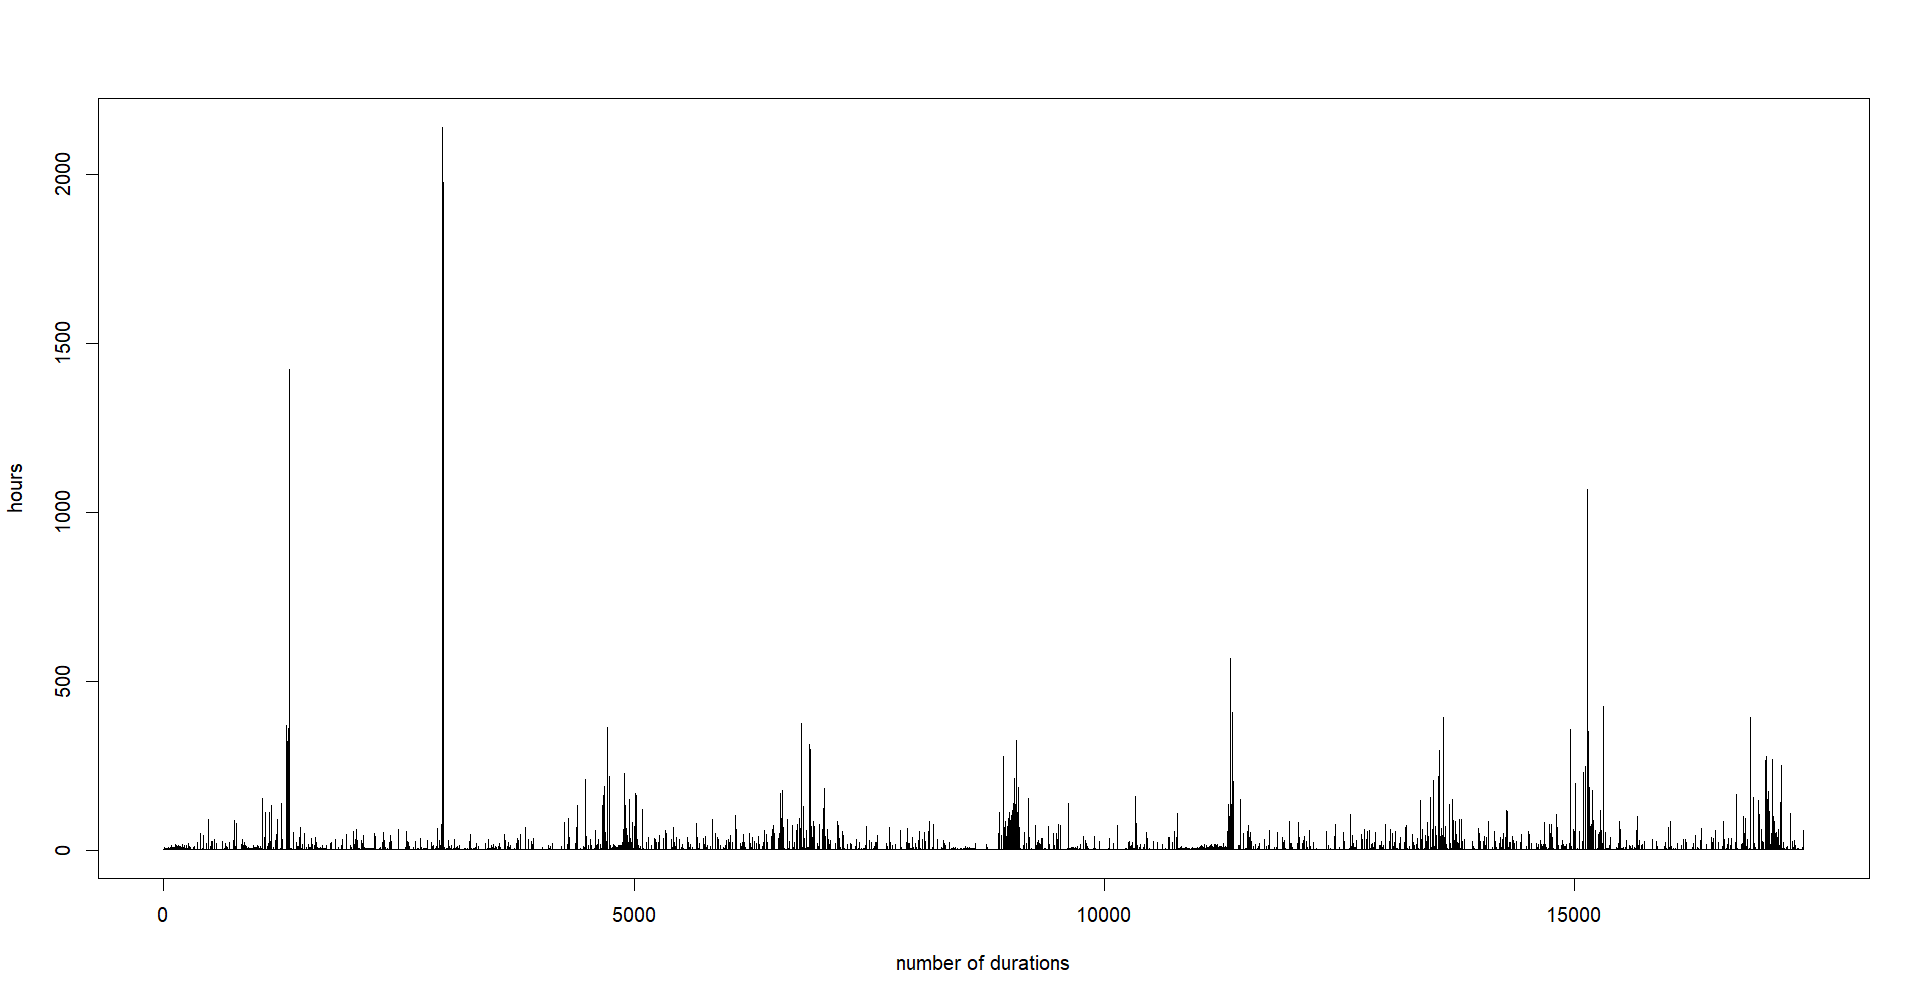
\includegraphics[width=0.85\linewidth]{dur_plot_2ft} \caption{Wave duration at 2ft threshold}\label{fig:2ft durations}
\end{figure}
\end{frame}

\begin{frame}{Plot of Durations (Cont..)}
\protect\hypertarget{plot-of-durations-cont..}{}
\begin{enumerate}
[1)]
\setcounter{enumi}{1}
\tightlist
\item
  Duration plot for the entire data based on 3ft threshold:
\end{enumerate}

\begin{figure}
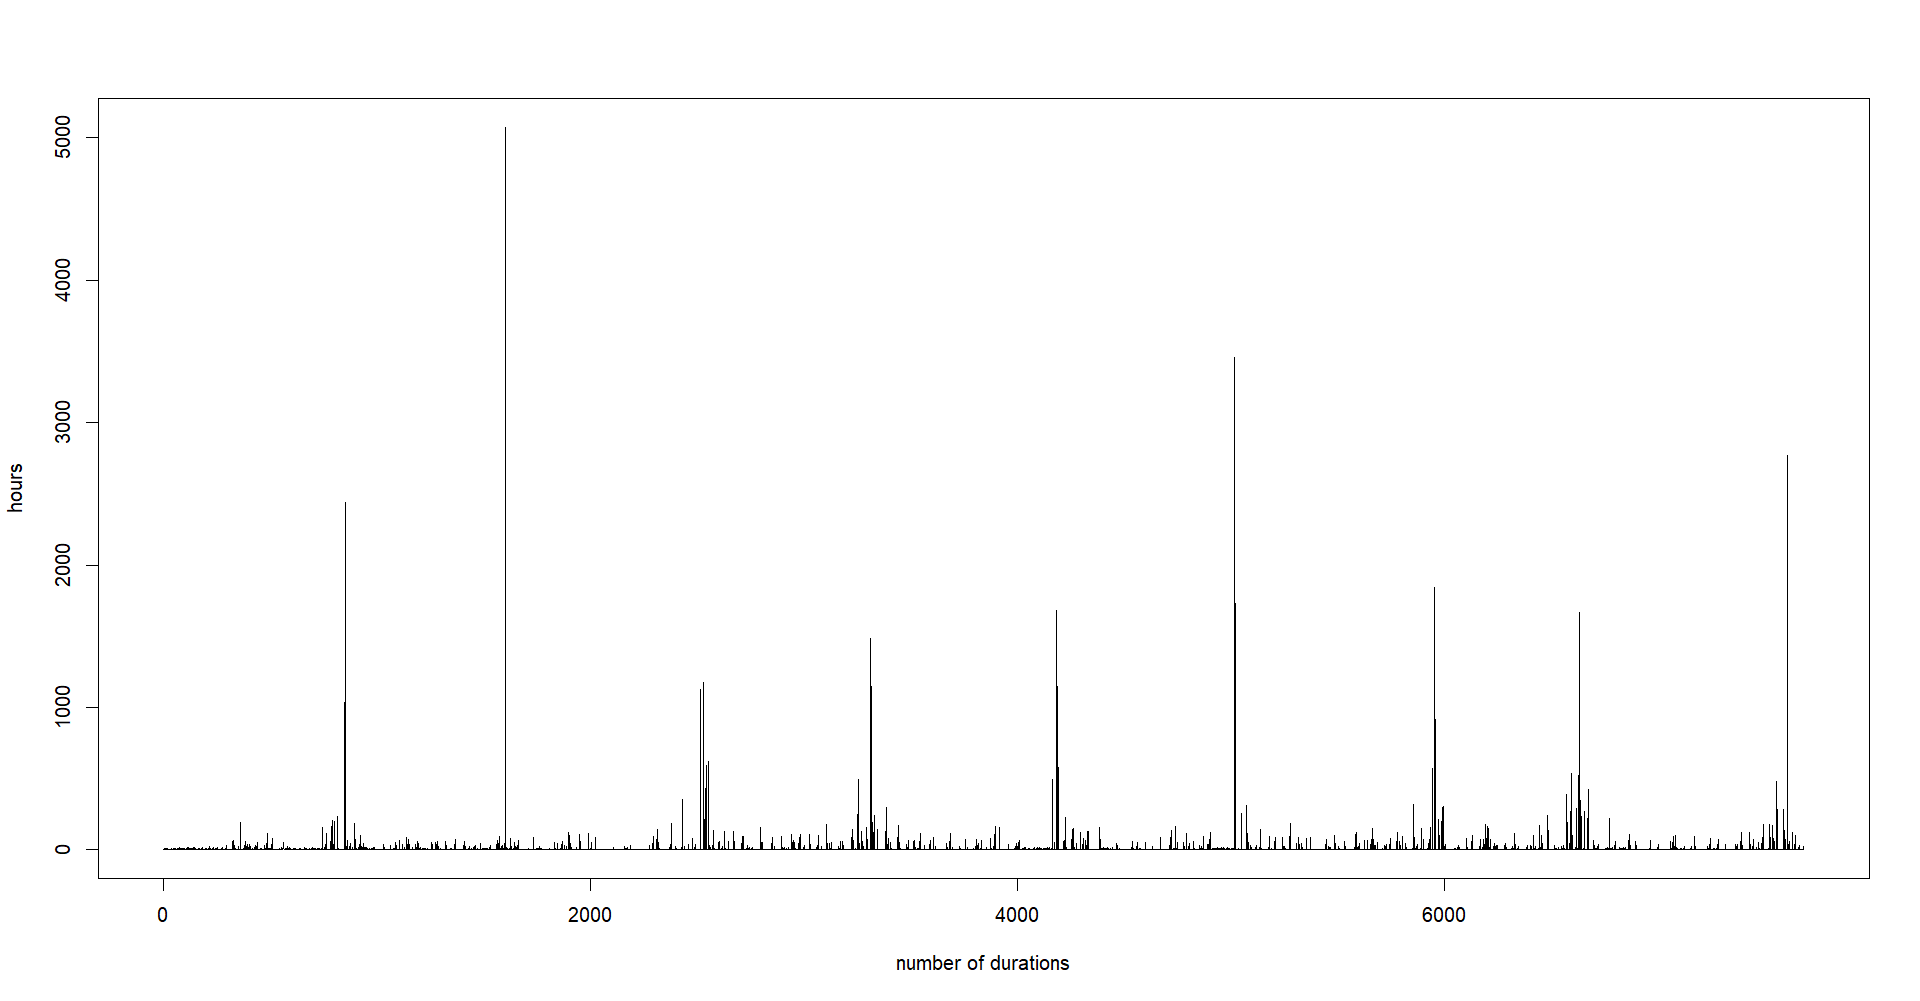
\includegraphics[width=0.85\linewidth]{dur_plot_3ft} \caption{Wave duration at 3ft threshold}\label{fig:3ft durations}
\end{figure}
\end{frame}

\begin{frame}{Plot of Durations (Cont..)}
\protect\hypertarget{plot-of-durations-cont..-1}{}
\begin{enumerate}
[1)]
\setcounter{enumi}{2}
\tightlist
\item
  Duration plot for the entire data based on 4ft threshold:
\end{enumerate}

\begin{figure}
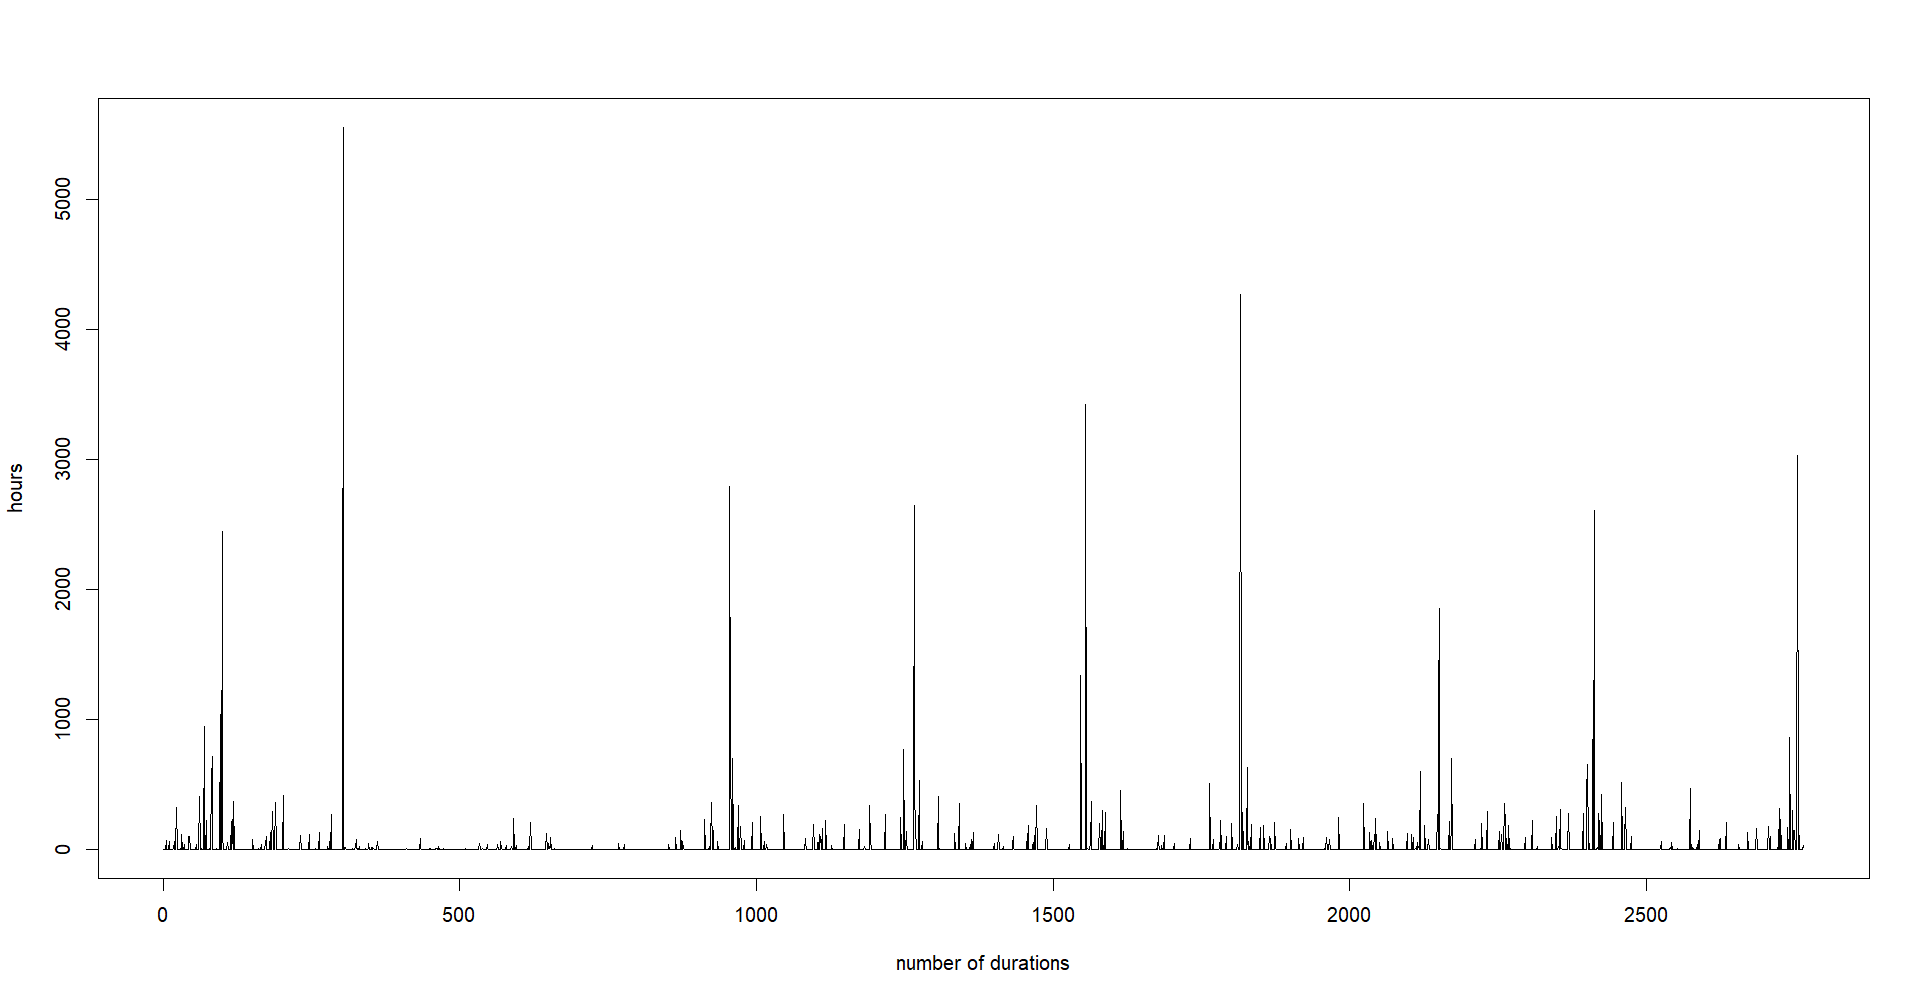
\includegraphics[width=0.85\linewidth]{dur_plot_4ft} \caption{Wave duration at 4ft threshold}\label{fig:4ft durations}
\end{figure}
\end{frame}

\begin{frame}{Plots based on Calm Season}
\protect\hypertarget{plots-based-on-calm-season}{}
\begin{enumerate}
[1)]
\tightlist
\item
  Duration plot for calm period based on 2ft threshold for the year
  2008:
\end{enumerate}

\begin{figure}
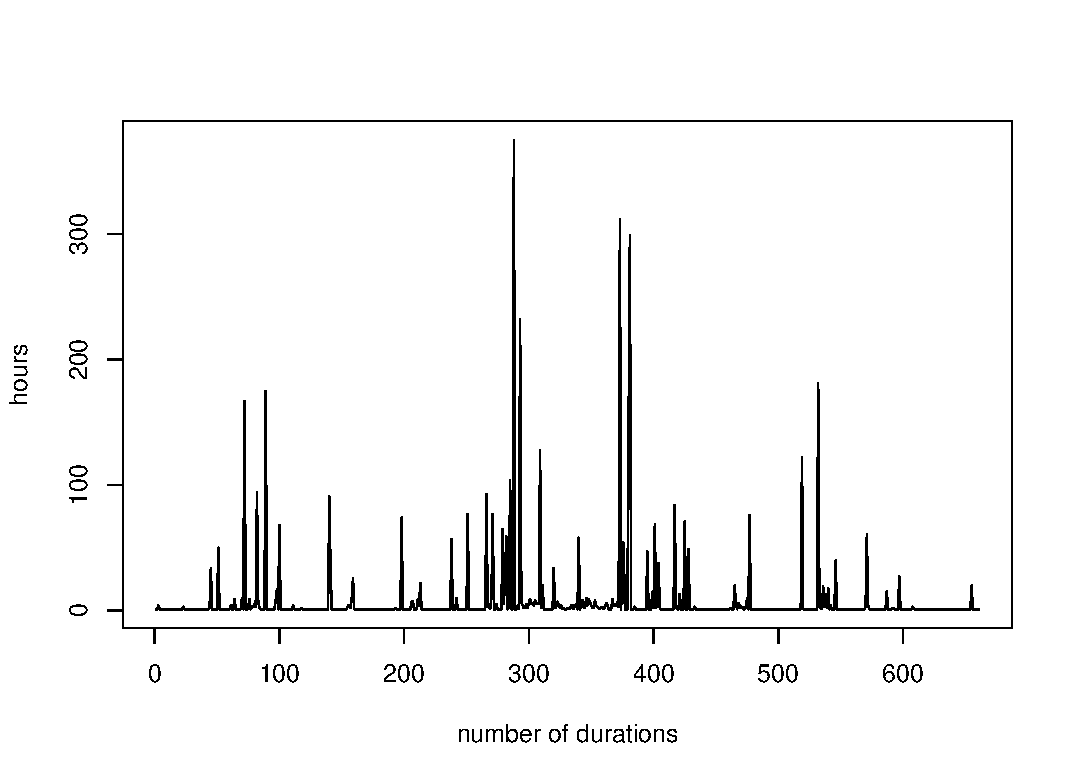
\includegraphics[width=0.8\linewidth]{Picture1} \caption{Wave duration of Calm Season for the year 2008}\label{fig:Calm Season}
\end{figure}
\end{frame}

\begin{frame}{Plots based on Windy Season}
\protect\hypertarget{plots-based-on-windy-season}{}
\begin{enumerate}
[1)]
\setcounter{enumi}{1}
\tightlist
\item
  Duration plot for Windy period based on 2ft threshold for the year
  2008:
\end{enumerate}

\begin{figure}
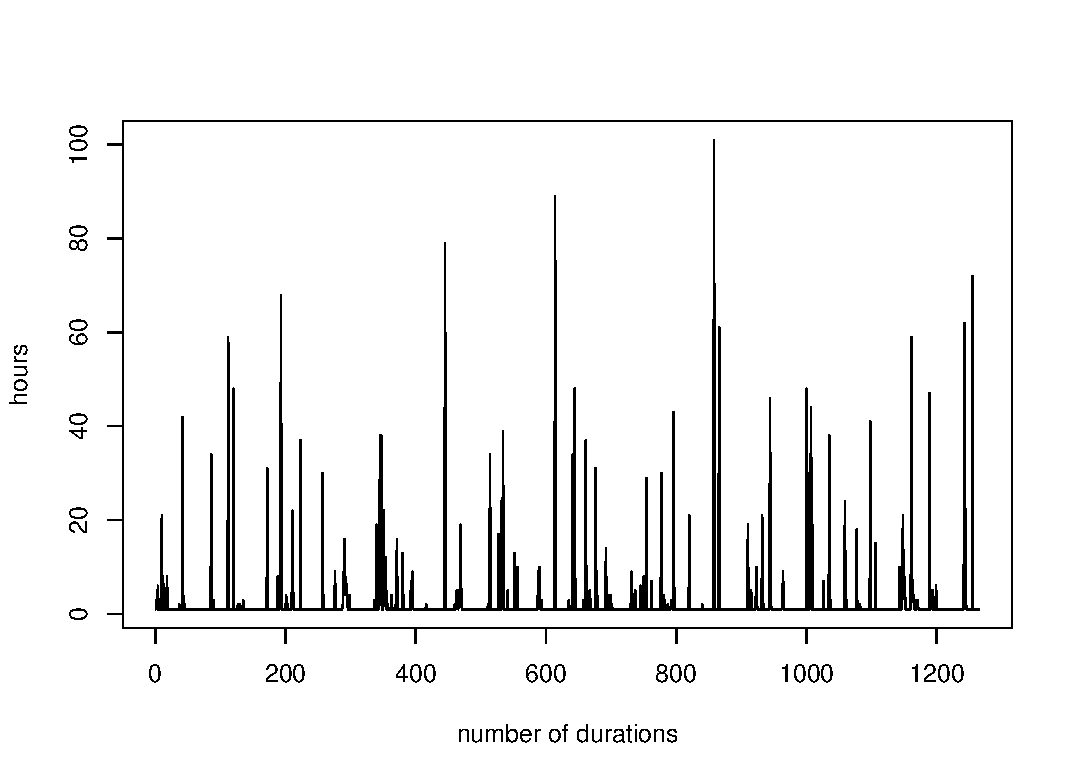
\includegraphics[width=0.8\linewidth]{Picture2} \caption{Wave duration of Windy Season for the year 2008}\label{fig:Windy Season}
\end{figure}
\end{frame}

\begin{frame}{Log-ACD Model with exogenous variables}
\protect\hypertarget{log-acd-model-with-exogenous-variables}{}
We define the durations \(x_i\) with exogenous variables as:

\(x_i = e^{\psi_i} \epsilon_i\) ;

where \(\epsilon_i\) are i.i.d with some density, and

\(\psi_i = \omega + \sum_{j=0}^m \alpha_j ln x_{i-j} + \sum_{j=0}^q \beta_j \psi_{i-j}+\sum_{j=1}^r\delta_jz_{i,j}\),

where \(z_{i,j}\) are the exogenous variables.

The exogenous variables used for modeling are
\textit{wind speed square},\(Z2, Z3, Z4\).

The missing data in the exogenous variables were backfilled.
\end{frame}

\begin{frame}{Procedure}
\protect\hypertarget{procedure}{}
\begin{itemize}
\item
  The first step was to identify the initial parameter values.
\item
  This was done using the properties of non-Gaussian autoregressive
  moving average (ARMA) models.
\item
  We first take the logarithmic transformation of the durations \(x_i\)
  and then fit an \(ARMA(Max(p,q),q)\) model to the log transformed
  durations.
\item
  Then based on the coefficients of the ARMA model we can obtain our
  initial value estimate.
\item
  This can be done using the \emph{arima} function in R using the
  \emph{method as CSS} which corresponds to minimizing the conditional
  sum-of-squares.
\end{itemize}
\end{frame}

\begin{frame}{Procedure (Cont..)}
\protect\hypertarget{procedure-cont..}{}
\begin{itemize}
\item
  The second step is to fit the model using the initial values we
  obtained for the parameters.
\item
  The final set of parameters are estimated using the conditional
  likelihood approach.
\item
  This can be done using the \emph{optim} function or \emph{nlminb}
  function in R.
\item
  The third step is to do a \emph{h-step} ahead forecast.
\item
  Then compute the Mean absolute percentage error (MAPE) for the
  forecasts.
\end{itemize}
\end{frame}

\begin{frame}{Simulation Study 1}
\protect\hypertarget{simulation-study-1}{}
Several simulation studies were conducted to see if the model was able
to return fitted values close to the values used to simulate the
datasets. All simulations are based on exponential distributions for the
errors.

\begin{table}[ht]
\caption{Results for Log-ACD(1,1)}
\begin{tabular}{lll}
 \hline
 Parameters& Simulated & Fitted \\
 \hline
 $\omega$   & 0.30 & 0.33 \\
 $\alpha_1$   & 0.20 & 0.17 \\
 $\beta_1$   & 0.70 & 0.65 \\
 $\delta_1$  & 0  & 0 \\
 \hline
\end{tabular}
\end{table}

The simulation results are based on average of 10 simulations of size
1500. Also note that the exogenous variables coefficient are considered
to be zero.
\end{frame}

\begin{frame}{Simulation Study 2}
\protect\hypertarget{simulation-study-2}{}
\begin{table}[ht]
\caption{Results for Log-ACD(1,1)}
\begin{tabular}{lll}
 \hline
 Parameters& Simulated & Fitted \\
 \hline
 $\omega$   & 0.30 & 0.31  \\
 $\alpha_1$   & 0.01 & 0.01  \\
 $\beta_1$  & 0.60 & 0.60  \\
 $\delta_1$   & 0.08 & 0.08  \\
 $\delta_2$   & -0.61 & -0.63  \\
 $\delta_3$   & 0.75 & 0.78   \\
 $\delta_4$   & -0.31 & -0.34 \\
 \hline
\end{tabular}
\end{table}

The simulation results are based on average of 100 simulations of size
1500.
\end{frame}

\begin{frame}{Simulation Study 3}
\protect\hypertarget{simulation-study-3}{}
\begin{table}[ht]
\caption{Results for Log-ACD(5,3)}
\begin{tabular}{lll}
 \hline
 Parameters& Simulated & Fitted \\
 \hline
 $\omega$   & 0.10 & 0.10  \\
 $\alpha_1$   & 0.10 & 0.10  \\
 $\alpha_2$  & 0.20 & 0.19  \\
 $\alpha_3$   & -0.10 & -0.11  \\
 $\alpha_4$   & 0.02 & 0.03  \\
 $\alpha_5$   & -0.15 & -0.15   \\
 $\beta_1$   & 0.70 & 0.74 \\
 $\beta_2$   & 0 & 0.01 \\
 $\beta_3$   & 0 & 0 \\
 $\delta_1$   & 0.05 & 0.05 \\
 \hline
\end{tabular}
\end{table}

The simulation results are based on average of 100 simulations of size
1500.
\end{frame}

\begin{frame}{Model fits}
\protect\hypertarget{model-fits}{}
All outputs are based on the durations computed for windy period for the
year 2010 with a threshold of 2ft.

\begin{table}[ht]
\caption{Results for Log-ACD(2,1) with no exogenous variables}
\begin{tabular}{lll}
 \hline
 Parameters & Initial & Fitted \\
 \hline
 $\omega$   & 0.01 & 0.21 \\
 $\alpha_1$    & 0.05 & -0.02 \\
 $\alpha_2$   & -0.01 & 0.09 \\
 $\beta_1$    & 0.95 & 0.85 \\
 $\delta_1$   & 0  & 0 \\
 \hline
\end{tabular}
\end{table}
\end{frame}

\begin{frame}{Model fits (Cont..)}
\protect\hypertarget{model-fits-cont..}{}
This table shows the reuslts based on the model using the four exogenous
variables: wind speed square, z2, z3 and z4.

\begin{table}[ht]
\caption{Results for Log-ACD(2,1) with exogenous variables}
\begin{tabular}{lll}
 \hline
 Parameters & Initial & Fitted  \\
 \hline
 $\omega$   & 0.03 & 0.23 \\
 $\alpha_1$   & 0.06 & 0.11 \\
 $\alpha_2$   & 0.03 & -0.02 \\
 $\beta_1$   & -0.11 & 0.20 \\
 $\delta_1$   & 0.45 & 0.40  \\
 $\delta_2$   & -1.19 & -1.26  \\
 $\delta_3$   & 1.18 & 1.24  \\
 $\delta_4$   & -0.31 & -0.35  \\
 \hline
\end{tabular}
\end{table}
\end{frame}

\begin{frame}{Forecast evaluation}
\protect\hypertarget{forecast-evaluation}{}
\begin{itemize}
\item
  The MAPE for 5-step ahead forecast for the model without exogenous
  variables was 23.33.
\item
  The MAPE for 5-step ahead forecast for the model with exogenous
  variables was 81.03.
\item
  We can see that the model without the exogenous variables have a lower
  MAPE compared to the model with the exogenous variables.
\item
  This may be because of the nature of exogenous variables.
\item
  We can see that the model is able to fit the durations well even for
  applications outside of financial domain.
\end{itemize}
\end{frame}

\begin{frame}{Summary}
\protect\hypertarget{summary}{}
\begin{itemize}
\item
  Duration models are a family of models based on ARCH/GARCH framework.
\item
  Instead of modeling the conditional variances we model the conditional
  mean of durations.
\item
  Duration models are very useful in studying irregularly spaced
  financial transaction level data.
\item
  Here we have shown several simulation study along with an example of
  fitting an duration model to a data outside of financial application
  by modeling wave height durations.
\end{itemize}
\end{frame}

\begin{frame}[allowframebreaks]{References}
\protect\hypertarget{references}{}
\hypertarget{refs}{}
\begin{CSLReferences}{1}{0}
\leavevmode\vadjust pre{\hypertarget{ref-EE}{}}%
Aerambamoorthy Thavaneswaran, You Liang, Nalini Ravishanker. 2015.
{``Generalized Duration Models and Optimal Estimation Using Estimating
Functions.''} \emph{Annals of the Institute of Statistical Mathematics}
67.

\leavevmode\vadjust pre{\hypertarget{ref-LogACD}{}}%
Bauwens, Luc, and Pierre Giot. 2000. {``The Logarithmic ACD Model: An
Application to the Bid-Ask Quote Process of Three NYSE Stocks.''}
\emph{Annales d'Économie Et de Statistique} 60.

\leavevmode\vadjust pre{\hypertarget{ref-SCD}{}}%
Bauwens, Luc, and David Veredas. 2004. {``The Stochastic Conditional
Duration Model: A Latent Variable Model for the Analysis of Financial
Durations.''} \emph{Econometrics eJournal} 119.

\leavevmode\vadjust pre{\hypertarget{ref-ACD}{}}%
Engle, Robert F., and Jeffrey R. Russell. 1998. {``Autoregressive
Conditional Duration: A New Model for Irregularly Spaced Transaction
Data.''} \emph{Econometrica} 66.

\leavevmode\vadjust pre{\hypertarget{ref-AACD}{}}%
Fernandes, Marcelo, and Joachim Grammig. 2006. {``A Family of
Autoregressive Conditional Duration Models.''} \emph{Journal of
Econometrics} 130.

\leavevmode\vadjust pre{\hypertarget{ref-FIACD}{}}%
Jasiak, Joann. 1999. {``Persistence in Intratrade Durations.''}
\emph{Capital Markets: Market Microstructure} 19.

\leavevmode\vadjust pre{\hypertarget{ref-ACDtext}{}}%
Tsay, R. 2009. \emph{Autoregressive Conditional Duration Models}.
\emph{Palgrave Handbook of Econometrics}. Vol. 2.

\end{CSLReferences}
\end{frame}

\end{document}
